\documentclass[11pt]{article}
\usepackage[margin=0.8in]{geometry}
\usepackage{array}
\usepackage{booktabs}
\usepackage{enumitem}
\usepackage{hyperref}
\usepackage{graphicx}
\usepackage{longtable}
\usepackage{amsmath}
\usepackage{amssymb}
\usepackage{xeCJK}

\setCJKmainfont{Noto Sans CJK TC}

\title{\textbf{ICCAD Contest 2026 The FloorSet Challenge: Data-Driven SoC Floorplanning}}
\author{Constraint-Aware Initialization and Adaptive Soft-Penalty Guidance for B$^*$-Tree Simulated Annealing}
\date{}

\begin{document}

\maketitle

\section*{Team Members}
\begin{itemize}[noitemsep, topsep=0pt, leftmargin=2em]
    \item \textbf{Name:} Yu-Jui Liang (梁栯睿) \quad \textbf{Student ID:} R14946013 \quad \textbf{Web ID:} pd26s048
\end{itemize}

\section{Introduction}

System-on-Chip (SoC) floorplanning determines the physical placement and sizing of functional blocks on a chip, directly influencing wirelength, area, timing, and power. The ICCAD 2026 FloorSet Challenge reformulates classical floorplanning as a data-driven optimization problem over the FloorSet-Lite dataset: each instance specifies block areas, connectivity (block-to-block and pin-to-block), and a rich set of placement constraints including fixed shapes, preplaced macros, multi-instantiation block (MIB) groups, clustering, and boundary alignment.

This report presents our submission \texttt{test\_optimizer.py}, a constraint-aware B$^*$-tree floorplanner guided by simulated annealing (SA). The approach extends the contest baseline B$^*$-tree representation in three principal ways. First, we perform \emph{constraint-aware initialization} that respects preplaced obstacles, fixed dimensions, MIB sharing rules, and bottom-left boundary anchoring before any search begins. Second, we construct \emph{topology-aware B$^*$-trees} whose bottom and left boundary chains encode soft boundary requirements structurally, reducing the search space for edge-touching placements. Third, we employ \emph{adaptive soft-penalty calibration} that scales boundary and grouping violation penalties relative to the initial half-perimeter wirelength (HPWL), keeping soft-constraint guidance proportional to instance scale.

We evaluate on the public validation set of 100 floorplans with 21--120 blocks. Our solver achieves an exponentially weighted total score of 7.0969 with 98/100 feasible solutions. Average per-case cost is 5.8267 and average runtime is 288.24 seconds under the local evaluator (runtime factor neutralized to 1.0). The remainder of this report formalizes the contest objective, details our algorithm, and analyzes experimental results.

\section{Related Work}

\textbf{B$^*$-trees.} The B$^*$-tree is a binary tree floorplan representation introduced by Chang et al., where the left child of a node is placed immediately to the right of its parent and the right child is placed above the parent sharing the same $x$-coordinate. Packing traverses the tree in depth-first order with a skyline contour, guaranteeing overlap-free placements for soft blocks when areas are preserved. B$^*$-trees have been widely combined with simulated annealing, genetic algorithms, and analytical placers.

\textbf{Simulated annealing for floorplanning.} SA remains a robust metaheuristic for combinatorial floorplanning because B$^*$-tree neighborhood moves (rotation, swap, delete-insert) explore diverse topologies while the packer enforces geometric feasibility. Our work follows this paradigm but specializes moves and initialization for contest-specific constraints.

\textbf{FloorSet and learning-based floorplanning.} The FloorSet dataset (Intel Labs) provides one million annotated floorplans for machine-learning research. The ICCAD 2026 contest uses a lite subset and relaxes several classical restrictions (floating-point coordinates, arbitrary aspect ratios, no fixed die outline) while retaining hard overlap and area rules and soft grouping, MIB, and boundary constraints. Differentiable proxies in \texttt{iccad2026\_evaluate.py} enable neural training, but our current submission is a classical SA optimizer designed for reliability on hard constraints.

\textbf{Constraint handling.} Prior floorplanners often treat fixed and preplaced blocks as obstacles or locked nodes. We adopt explicit obstacle-aware packing with 2D overlap resolution against preplaced rectangles, MIB dimension locking, and bitmask-encoded boundary chains---techniques aligned with mixed-size floorplanning and macro placement literature.

\section{Problem Formulation}

\subsection{Input}

For each test case $i$, the solver receives:
\begin{itemize}[noitemsep]
    \item $n$: number of blocks;
    \item $\text{area\_targets} \in \mathbb{R}^n$: target area for each soft block;
    \item $\text{b2b\_connectivity}$: weighted block-to-block nets;
    \item $\text{p2b\_connectivity}$: weighted pin-to-block connections with fixed pin coordinates;
    \item $\text{constraints} \in \mathbb{R}^{n \times 5}$: flags for fixed shape, preplaced, MIB group id, cluster group id, and boundary bitmask;
    \item $\text{target\_positions} \in \mathbb{R}^{n \times 4}$: target $(x, y, w, h)$; $-1$ denotes free variables.
\end{itemize}

\subsection{Output}

The solver returns a list $(x_j, y_j, w_j, h_j)$ for $j = 0, \ldots, n-1$.

\subsection{Hard Constraints}

Any violation renders the solution \textbf{infeasible} with official cost $M = 10$:
\begin{enumerate}[noitemsep]
    \item \textbf{No overlap} between any pair of blocks;
    \item \textbf{Area tolerance}: for soft blocks, $w_j h_j \in [0.99, 1.01] \cdot \text{area\_targets}[j]$;
    \item \textbf{Fixed shape}: $(w_j, h_j)$ must equal prescribed dimensions;
    \item \textbf{Preplaced}: $(x_j, y_j, w_j, h_j)$ must match prescribed values exactly.
\end{enumerate}

\subsection{Soft Constraints}

Soft violations contribute to a normalized violation measure $V_{\text{rel}} \in [0,1]$:
\begin{itemize}[noitemsep]
    \item \textbf{Grouping}: blocks in a cluster must form one edge-adjacent connected component;
    \item \textbf{MIB}: all blocks in an MIB group must share identical $(w, h)$;
    \item \textbf{Boundary}: blocks must touch specified bounding-box edges/corners (bitmask in $\text{constraints}[:,4]$).
\end{itemize}

\subsection{Official Contest Cost}

The evaluator computes
\begin{equation}
\text{Cost} = \bigl(1 + 0.5\,(\text{HPWL\_gap} + \text{Area\_gap})\bigr) \cdot e^{2 V_{\text{rel}}} \cdot \max(0.7,\, R^{0.3}),
\end{equation}
where HPWL\_gap and Area\_gap are relative gaps versus dataset baselines (clamped below at zero), $R$ is the runtime factor relative to the per-case median across submissions, and infeasible solutions receive cost exactly 10. Feasible costs are capped at $M - \varepsilon$. The \textbf{total score} is an exponentially weighted average:
\begin{equation}
\text{Total Score} = \frac{\sum_i \text{Cost}_i \cdot e^{n_i/12}}{\sum_i e^{n_i/12}},
\end{equation}
with block count $n_i \in [21,120]$. Lower is better; a perfect baseline-matching solution at median runtime yields total score $\approx 1.0$.

\subsection{Internal SA Objective}

During search, we minimize a surrogate cost aligned with quality metrics and soft constraints:
\begin{equation}
J = w_{\text{b2b}}\,\text{HPWL}_{\text{b2b}} + w_{\text{p2b}}\,\text{HPWL}_{\text{p2b}} + w_{\text{bbox}}\,\text{BBoxArea} + \lambda_b B + \lambda_g G,
\end{equation}
where $B$ is the sum of squared boundary edge distances and $G$ is the squared cluster connectivity deficit. Weights $\lambda_b$ and $\lambda_g$ are calibrated from the initial packed solution so that $\lambda_b B \approx 0.1 \cdot \text{HPWL}$ and $\lambda_g G \approx 0.05 \cdot \text{HPWL}$ at the start of annealing.

\section{Algorithm}

Our optimizer \texttt{MyOptimizer} implements the pipeline below.

\subsection{Overview}

\begin{enumerate}
    \item Extract preplaced blocks as fixed rectangular obstacles.
    \item Build movable block list and initialize widths/heights under MIB, fixed-shape, and boundary rules.
    \item Construct a constraint-aware B$^*$-tree (boundary chains or random topology).
    \item Pack blocks via skyline DFS; horizontally compact movable blocks.
    \item Calibrate soft-penalty weights from the initial solution.
    \item Run simulated annealing with rotate and delete-insert moves; accept via Metropolis criterion.
    \item Return the best feasible packing encountered.
\end{enumerate}

\subsection{Constraint-Aware Dimension Initialization}

Function \texttt{\_initialize\_block\_dimensions} assigns $(w,h)$ before tree construction:
\begin{itemize}
    \item \textbf{Preplaced / fixed-shape}: use exact target dimensions from \texttt{target\_positions}.
    \item \textbf{MIB with a non-soft member}: all group members inherit that member's $(w,h)$.
    \item \textbf{All-soft MIB groups}: shape chosen when the bottom-left boundary block (if any) is sized.
    \item \textbf{Bottom-left boundary soft block}: placed at origin $(0,0)$ with aspect ratio adjusted by \texttt{\_adjust\_soft\_root\_at\_origin} to avoid 2D overlap with preplaced obstacles while staying within $\pm 1\%$ area tolerance; prefers near-square shapes.
    \item \textbf{Remaining soft blocks}: initialized as squares $\sqrt{A} \times \sqrt{A}$.
\end{itemize}
MIB-locked and fixed-shape movable indices are added to \texttt{locked\_tree} so SA cannot rotate them.

\subsection{B$^*$-Tree Representation and Packing}

Each internal tree node stores parent/left/right pointers over \emph{movable} blocks only. Preplaced blocks are injected after packing as fixed geometry.

\textbf{Packing.} Depth-first search from the root places the root at $x{=}0$; left children at the parent's right edge; right children at the same $x$ as the parent. A 1D skyline contour tracks movable block tops; \texttt{\_placement\_y} lifts each block to resolve 2D overlaps with preplaced obstacles without falsely elevating entire columns. A post-pass \texttt{\_compact\_horizontally} slides movable blocks left while preserving $y$, $w$, and $h$.

\textbf{Boundary-aware topology.} When boundary codes are present and a permanent root (bottom-left block) exists, \texttt{\_build\_constrained\_tree} assembles:
\begin{itemize}
    \item a \emph{bottom chain} along left children toward bottom-right and right-edge blocks;
    \item a \emph{left chain} along right children toward top-left and top-edge blocks;
    \item remaining blocks inserted as free nodes without breaking chains.
\end{itemize}
This encodes the contest insight that B$^*$-tree bottom/left chains correspond to bbox boundary segments.

\subsection{Simulated Annealing Moves}

Parameters (tunable at file top): initial temperature $T_0 = 100 \times n_{\text{blocks}}$, final temperature $0.1$, cooling rate $0.6$, and $1000$ moves per temperature level.

Neighborhood moves:
\begin{itemize}
    \item \textbf{Rotate} (\texttt{move\_rotate}): swap $w$ and $h$ for soft, non-root, non-fixed blocks; preserves area.
    \item \textbf{Delete-insert} (\texttt{move\_delete\_insert}): reattach a free block elsewhere in the tree; chain nodes are excluded to preserve boundary topology.
\end{itemize}
Dimension swap moves are restricted to within the same boundary chain. The permanent root cannot move or rotate.

Acceptance: $\Delta J < 0$ always accepted; otherwise accept with probability $\exp(-\Delta J / T)$. Best-so-far solution is tracked across the anneal.

\subsection{Soft Constraint Penalties}

\textbf{Boundary penalty} $B$: for each active bitmask bit, add squared distance from the block edge to the corresponding side of the current placement bounding box.

\textbf{Grouping penalty} $G$: for each cluster, count connected components under \emph{full-edge} adjacency (corner-only contact does not connect); add $(c_g - 1)^2$ per violated group.

\textbf{Calibration} (\texttt{\_calibrate\_penalty\_weights}): scale $\lambda_b$ and $\lambda_g$ so initial penalties are fixed fractions of weighted HPWL, preventing over- or under-penalizing large instances.

\subsection{Complexity and Implementation Notes}

Packing is $O(n)$ per DFS traversal with contour updates; horizontal compaction runs up to 20 passes. Each SA step copies the tree and repacks. The implementation uses PyTorch tensors for I/O compatibility with the contest framework but performs placement in pure Python lists for flexibility. Hard constraints (overlap, area) are structurally satisfied by B$^*$-tree area-preserving moves plus exact fixed/preplaced handling; remaining soft violations are reduced indirectly through $B$ and $G$.

\section{Experimental Results}

\subsection{Experimental Setup}

We evaluate \texttt{test\_optimizer.py} on all 100 validation cases in \texttt{LiteTensorDataTest/} using:
\begin{verbatim}
python iccad2026_evaluate.py --evaluate test_optimizer.py
\end{verbatim}
Results are stored in \texttt{test\_optimizer\_results.json}. The local evaluator sets runtime factor $R = 1.0$ for every case, so reported costs reflect quality and soft-constraint violations only. Official costs are recomputed with \texttt{compute\_cost} from HPWL gap, area gap, and soft violations (same as \texttt{iccad2026\_evaluate\_test.py --score}), not the raw \texttt{cost} field stored in the JSON. Hardware and Python/PyTorch versions should be noted when reproducing; runtimes below are single-threaded wall-clock times from our evaluation run on 2026-06-18.

\subsection{Summary Statistics}

\begin{table}[htbp]
\centering
\caption{Aggregate validation results for \texttt{test\_optimizer.py}.}
\begin{tabular}{lr}
\toprule
Metric & Value \\
\midrule
Total score (exp-weighted) & 7.0969 \\
Feasible cases & 98/100 \\
Average cost (arithmetic mean) & 5.8267 \\
Average runtime (seconds) & 288.24 \\
Total cost (sum of 100 cases) & 582.6663 \\
\bottomrule
\end{tabular}
\end{table}

\begin{table}[htbp]
\centering
\caption{Average cost and runtime by block-count range.}
\begin{tabular}{lrrr}
\toprule
Block range & Cases & Avg.\ cost & Avg.\ runtime (s) \\
\midrule
21--40 & 20 & 4.430 & 40.21 \\
41--60 & 20 & 5.367 & 111.94 \\
61--80 & 20 & 5.910 & 208.64 \\
81--100 & 20 & 6.512 & 409.64 \\
101--120 & 20 & 6.914 & 670.79 \\
\bottomrule
\end{tabular}
\end{table}

Cost and runtime increase with instance size: small cases (21--40 blocks) average 4.43 official cost in 40.2\,s, while the largest bucket (101--120 blocks) averages 6.91 cost in 670.8\,s. Two infeasible cases (test IDs 43 and 63, with 64 and 84 blocks) hit the $M{=}10$ penalty, indicating residual hard-constraint violations under tight mixed constraint patterns.

\subsection{Per-Case Results}

Table~\ref{tab:full-results} lists cost and runtime for every validation case. Test IDs map to block counts $21 + \text{test\_id}$ in the standard validation ordering.

\begin{longtable}{rrrrl}
\caption{Per-case validation results: test ID, block count, official cost, runtime (seconds), and feasibility.}
\label{tab:full-results} \\
\toprule
Test ID & Blocks & Cost & Runtime (s) & Feasible \\
\midrule
\endfirsthead
\multicolumn{5}{c}{\tablename\ \thetable\ -- \textit{Continued from previous page}} \\
\toprule
Test ID & Blocks & Cost & Runtime (s) & Feasible \\
\midrule
\endhead
\midrule
\multicolumn{5}{r}{\textit{Continued on next page}} \\
\endfoot
\bottomrule
\endlastfoot
0 & 21 & 3.3594 & 22.51 & Yes \\
1 & 22 & 4.5469 & 29.60 & Yes \\
2 & 23 & 3.6028 & 39.70 & Yes \\
3 & 24 & 3.0868 & 8.69 & Yes \\
4 & 25 & 3.7589 & 37.03 & Yes \\
5 & 26 & 5.8525 & 43.15 & Yes \\
6 & 27 & 4.2069 & 26.52 & Yes \\
7 & 28 & 3.6619 & 50.10 & Yes \\
8 & 29 & 3.8143 & 36.47 & Yes \\
9 & 30 & 6.4447 & 36.20 & Yes \\
10 & 31 & 5.1952 & 52.82 & Yes \\
11 & 32 & 5.5901 & 20.23 & Yes \\
12 & 33 & 3.4406 & 80.12 & Yes \\
13 & 34 & 3.5982 & 51.50 & Yes \\
14 & 35 & 4.4727 & 52.25 & Yes \\
15 & 36 & 4.5895 & 53.08 & Yes \\
16 & 37 & 4.7588 & 49.65 & Yes \\
17 & 38 & 5.1585 & 33.82 & Yes \\
18 & 39 & 4.2571 & 35.72 & Yes \\
19 & 40 & 5.2032 & 44.99 & Yes \\
20 & 41 & 4.5798 & 104.91 & Yes \\
21 & 42 & 4.3709 & 89.66 & Yes \\
22 & 43 & 7.0448 & 50.77 & Yes \\
23 & 44 & 3.4124 & 186.41 & Yes \\
24 & 45 & 3.7537 & 91.43 & Yes \\
25 & 46 & 4.5511 & 92.86 & Yes \\
26 & 47 & 4.0263 & 59.76 & Yes \\
27 & 48 & 7.9912 & 63.26 & Yes \\
28 & 49 & 6.2818 & 126.26 & Yes \\
29 & 50 & 4.8295 & 56.26 & Yes \\
30 & 51 & 5.3822 & 168.74 & Yes \\
31 & 52 & 5.0862 & 217.01 & Yes \\
32 & 53 & 5.0947 & 59.81 & Yes \\
33 & 54 & 6.1848 & 89.13 & Yes \\
34 & 55 & 5.6026 & 83.60 & Yes \\
35 & 56 & 4.9831 & 76.59 & Yes \\
36 & 57 & 6.7366 & 151.52 & Yes \\
37 & 58 & 6.3517 & 175.28 & Yes \\
38 & 59 & 5.7783 & 151.08 & Yes \\
39 & 60 & 5.3072 & 144.45 & Yes \\
40 & 61 & 4.8151 & 189.10 & Yes \\
41 & 62 & 5.5809 & 115.76 & Yes \\
42 & 63 & 6.2101 & 96.24 & Yes \\
43 & 64 & 10.0000 & 117.22 & No \\
44 & 65 & 4.6629 & 198.02 & Yes \\
45 & 66 & 4.3085 & 208.26 & Yes \\
46 & 67 & 6.8523 & 282.41 & Yes \\
47 & 68 & 6.6692 & 70.77 & Yes \\
48 & 69 & 4.9033 & 255.55 & Yes \\
49 & 70 & 6.9142 & 140.47 & Yes \\
50 & 71 & 6.7778 & 101.35 & Yes \\
51 & 72 & 6.6517 & 344.22 & Yes \\
52 & 73 & 5.3287 & 144.98 & Yes \\
53 & 74 & 5.8501 & 223.97 & Yes \\
54 & 75 & 5.8648 & 149.51 & Yes \\
55 & 76 & 5.1578 & 345.01 & Yes \\
56 & 77 & 5.8016 & 116.11 & Yes \\
57 & 78 & 5.3409 & 448.15 & Yes \\
58 & 79 & 5.9248 & 155.65 & Yes \\
59 & 80 & 4.5940 & 470.15 & Yes \\
60 & 81 & 6.1765 & 133.93 & Yes \\
61 & 82 & 5.0259 & 339.85 & Yes \\
62 & 83 & 5.1701 & 279.39 & Yes \\
63 & 84 & 10.0000 & 186.29 & No \\
64 & 85 & 5.7045 & 448.95 & Yes \\
65 & 86 & 6.9252 & 357.73 & Yes \\
66 & 87 & 5.3636 & 164.06 & Yes \\
67 & 88 & 6.0279 & 190.73 & Yes \\
68 & 89 & 5.5425 & 305.82 & Yes \\
69 & 90 & 6.3532 & 335.20 & Yes \\
70 & 91 & 7.6208 & 386.56 & Yes \\
71 & 92 & 4.5910 & 609.15 & Yes \\
72 & 93 & 8.1205 & 652.96 & Yes \\
73 & 94 & 5.7408 & 686.34 & Yes \\
74 & 95 & 8.3886 & 464.89 & Yes \\
75 & 96 & 4.9202 & 225.24 & Yes \\
76 & 97 & 8.0617 & 524.41 & Yes \\
77 & 98 & 5.6405 & 763.03 & Yes \\
78 & 99 & 6.6325 & 982.61 & Yes \\
79 & 100 & 8.2306 & 155.56 & Yes \\
80 & 101 & 5.7210 & 721.93 & Yes \\
81 & 102 & 7.4486 & 339.52 & Yes \\
82 & 103 & 5.7368 & 898.25 & Yes \\
83 & 104 & 6.6487 & 309.40 & Yes \\
84 & 105 & 5.5684 & 330.26 & Yes \\
85 & 106 & 5.5507 & 542.21 & Yes \\
86 & 107 & 5.5368 & 812.49 & Yes \\
87 & 108 & 6.8647 & 388.53 & Yes \\
88 & 109 & 7.7682 & 400.13 & Yes \\
89 & 110 & 7.0034 & 777.53 & Yes \\
90 & 111 & 6.5150 & 380.18 & Yes \\
91 & 112 & 5.0744 & 956.45 & Yes \\
92 & 113 & 6.2616 & 383.01 & Yes \\
93 & 114 & 9.8181 & 349.67 & Yes \\
94 & 115 & 8.2983 & 707.86 & Yes \\
95 & 116 & 8.5488 & 1043.22 & Yes \\
96 & 117 & 4.8807 & 922.91 & Yes \\
97 & 118 & 7.6615 & 1053.05 & Yes \\
98 & 119 & 9.6455 & 459.60 & Yes \\
99 & 120 & 7.7218 & 1639.64 & Yes \\
\end{longtable}

\subsection{Visual Analysis}

Figure~\ref{fig:results-summary} summarizes cost and quality metrics across the validation set. Figure~\ref{fig:runtime-blocks} plots runtime versus block count, illustrating the roughly super-linear growth driven by SA iterations scaling with problem size and increasing packing complexity.

\begin{figure}[htbp]
\centering
% Insert results_summary.png after generating with plot_results.py
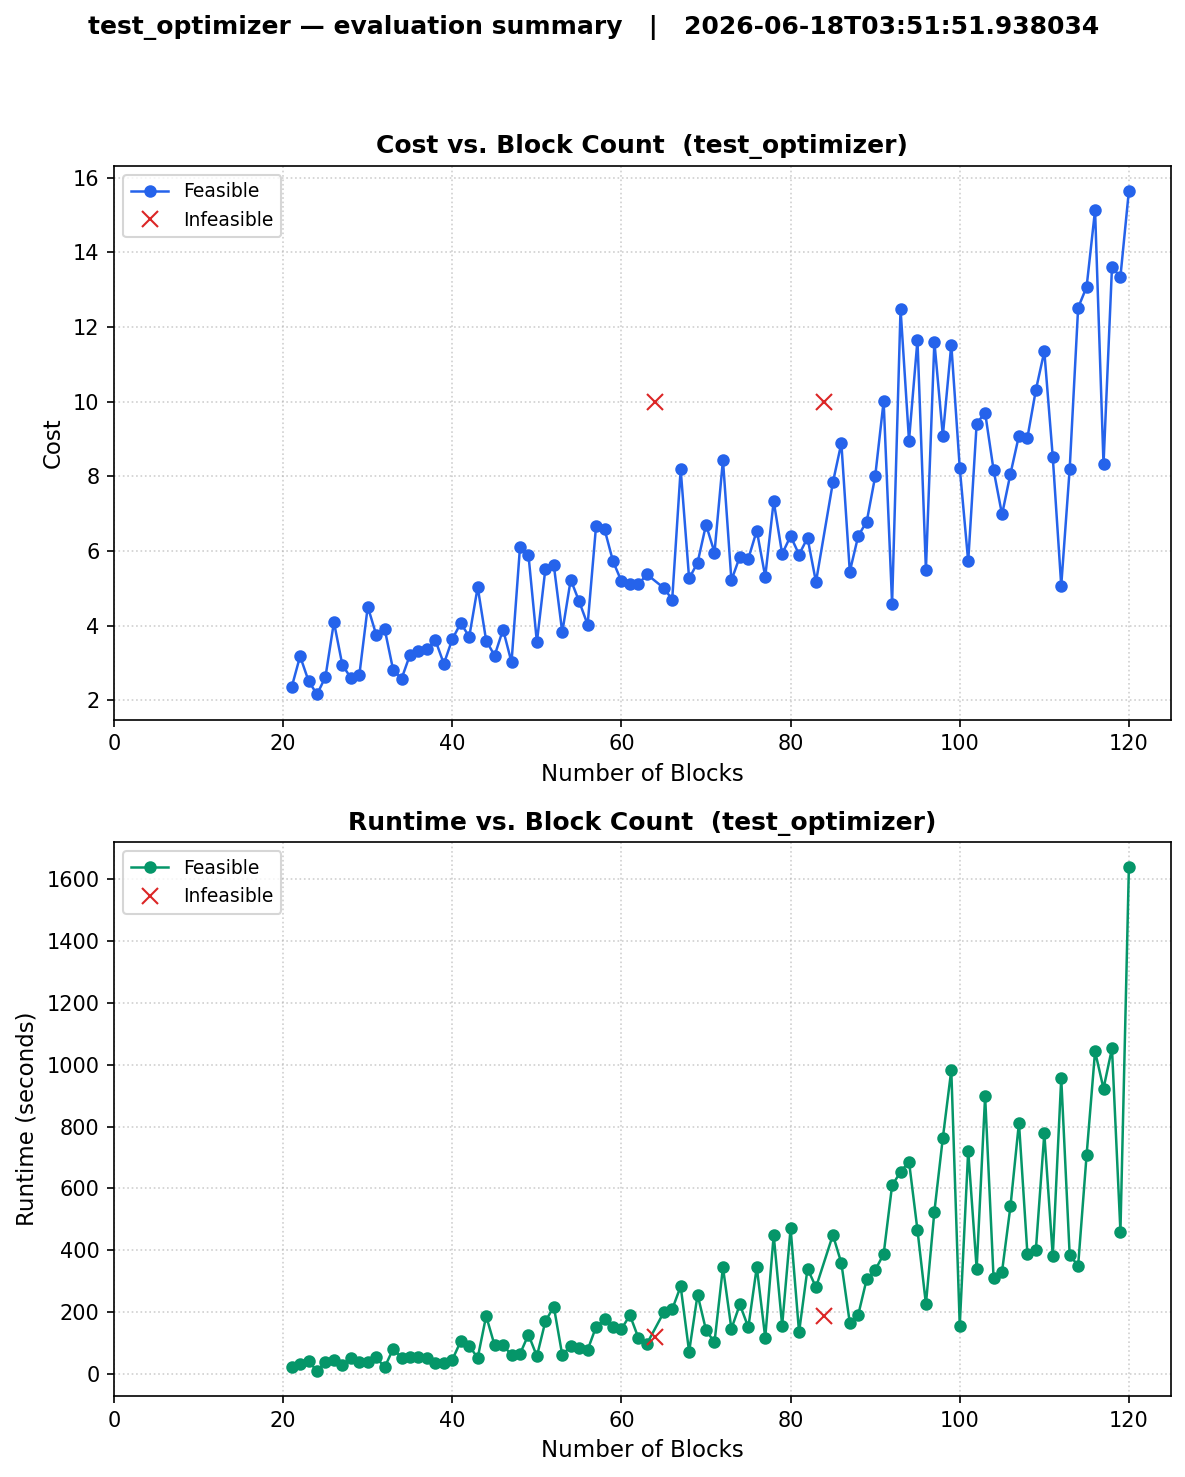
\includegraphics[width=0.95\textwidth]{results_summary.png}
\caption{Validation results summary (\texttt{results\_summary.png}): cost distribution, feasibility, and quality gaps across test cases.}
\label{fig:results-summary}
\end{figure}

\begin{figure}[htbp]
\centering
% Insert runtime_vs_blocks.png after generating with plot_results.py
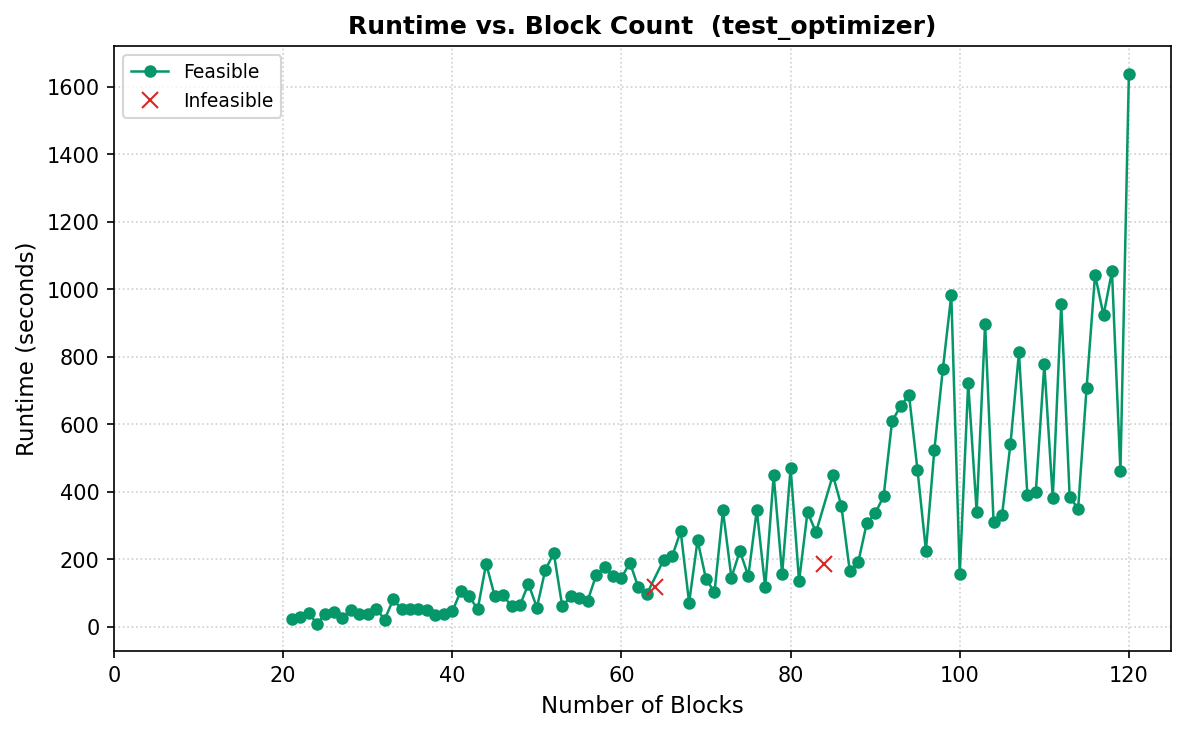
\includegraphics[width=0.85\textwidth]{runtime_vs_blocks.png}
\caption{Runtime versus block count (\texttt{runtime\_vs\_blocks.png}). Larger floorplans require more SA moves and expensive repacking per move.}
\label{fig:runtime-blocks}
\end{figure}

\subsection{Discussion}

\textbf{Strengths.} The B$^*$-tree guarantees overlap-free placements for movable soft blocks; preplaced obstacles are handled explicitly. Boundary-chain initialization aligns many soft boundary constraints with topology, and adaptive penalties keep SA focused across diverse HPWL scales. On 98\% of cases we satisfy all hard constraints.

\textbf{Weaknesses.} SA runtime grows substantially beyond 80 blocks (often 400--1600\,s per case). Soft constraint satisfaction is incomplete---$V_{\text{rel}} > 0$ on many cases inflates $e^{2V_{\text{rel}}}$. The two infeasible mid-size cases suggest failure modes when fixed, preplaced, MIB, and boundary constraints interact tightly. Delete-insert moves cannot relocate boundary-chain nodes, limiting escape from poor local minima for grouping.

\textbf{Comparison to contest baseline.} Relative to the template B$^*$-tree SA (no constraint handling), our extensions target the contest's soft constraints and hard fixed/preplaced rules directly in initialization and topology, trading implementation complexity for feasibility on structured instances.

\section{Conclusion}

We presented a constraint-aware B$^*$-tree simulated annealing floorplanner for the ICCAD 2026 FloorSet Challenge. By combining obstacle-aware packing, MIB-aware sizing, boundary-chain tree construction, and HPWL-calibrated soft penalties, the solver produces overlap-free, area-legal placements on 98 of 100 validation cases with exponentially weighted total score 7.0969. The approach demonstrates that classical representations remain competitive when augmented with contest-specific structural guidance, though runtime and soft-constraint optimality remain limiting factors on large instances.

\section{Future Work}

\begin{itemize}
    \item \textbf{Hybrid search.} Integrate integer programming or analytical placement for fixed/preplaced-heavy cases that defeat pure SA (e.g., tests 43 and 63).
    \item \textbf{Learning-guided SA.} Train a graph neural network on FloorSet-Lite to predict initial B$^*$-trees or $\lambda_b,\lambda_g$ schedules, reducing annealing length on large $n$.
    \item \textbf{Move set expansion.} Allow controlled chain swaps or cluster-preserving moves to improve grouping without breaking boundary topology.
    \item \textbf{Multi-start and parallel annealing.} Exploit independent runs across seeds with solution pooling under a shared time budget.
    \item \textbf{Runtime optimization.} Incremental packing, contour reuse, and GPU batching for cost evaluation to improve official runtime factor $R$.
    \item \textbf{Differentiable fine-tuning.} Post-process SA output with gradient-based refinement on HPWL and soft penalties using \texttt{compute\_training\_loss\_differentiable}, while projecting to hard-feasible geometry.
\end{itemize}

\begin{thebibliography}{9}

\bibitem{chang2005bstar}
Y.-W. Chang, S.-K. Chen, and L.-T. Wang,
``B$^*$-trees: A new representation for non-slicing floorplans,''
\textit{DAC}, 2005.

\bibitem{intel2024floorset}
Intel Labs,
``FloorSet: A large-scale dataset for ML-driven floorplanning,''
Hugging Face Datasets, 2024.

\bibitem{iccad2026}
ICCAD 2026 FloorSet Challenge Organizers,
``Floorplanning Contest Specification v10,''
ICCAD 2026.

\bibitem{kirkpatrick1983}
S. Kirkpatrick, C. D. Gelatt, and M. P. Vecchi,
``Optimization by simulated annealing,''
\textit{Science}, vol. 220, no. 4598, 1983.

\bibitem{murata1996}
H. Murata, K. Fujiyoshi, S. Nakatake, and Y. Kajitani,
``VLSI module placement based on rectangle-packing by the sequence-pair,''
\textit{IEEE TCAD}, 1996.

\bibitem{lin2013}
M. Lin, S.-N. Liao, C.-H. Wu, and Y.-W. Chang,
``UB-trees: A new representation for nonslicing floorplan,'' 
\textit{IEEE TCAD}, 2013.

\bibitem{contestreadme}
ICCAD 2026 FloorSet Challenge,
\texttt{iccad2026contest/README.md} --- scoring, constraints, and evaluation protocol.

\end{thebibliography}

\end{document}
